\chapter{Hardware-Anpassungen}

\section{Piplinestufe für Adressports}
Da der Verwendete Prozessor Adress-Isolation (siehe Kapitel \ref{subsec:add_iso}) einsetzt, sollten die Adressen so lange an einem Port anliegen bis diese geändert werden.
Die für die Schreib- und Lesezugriffe verwendeten Adressen werden jeweils zwischen den Takten von dem Adress-Decoder berechnet und an die benötigten Ports angelegt. Dadurch ist gewährleistet, dass diese mit der steigenden Taktflanke auch übernommen werden können. Die Auswahl der Ports wird über Enable-Signale geregelt. Im Fall dieser Architektur treten in diesem Fall Glitches auf, die auf Grund der unterschiedlichen Berechnungszeiten der Kombinatorik verursacht werden. In Schaubild \ref{fig:glitches} wird dieses Verhalten veranschaulicht. Hier ist zu erkennen, dass das Enable-Signal vor schaltet bevor die neue Adresse angelegt wird. Dadurch wird ein Glitch in den Adressleitungen verursacht. Dieses Szenario tritt nur auf, wenn ein Wechsel in den Enable-Signalen und sich somit die Herkunft der Adressen geändert wird.
% Werden beispielsweise zwei Instruktionen verwendet die beide an Register-File 1 schreiben, so werden die entsprechenden Adressen an die Ports 0 und 1 angelegt. Sobald diese zu Verfügung stehen, werden diese von den Enable-Signalen freigegeben.\\

\begin{figure}[H] 
	\centering
	\includesvg[width=0.70\textwidth]{glitches}
	\caption{Glitches Write-Adress}
	\label{fig:glitches}
\end{figure}


% Dies liegt daran, dass die benötigten Enable-Signale aufwendig berechnet werden müssen und dies eine kurze Verzögerung nach sich zieht
Das beschriebene Problem verursacht eine Erhöhung der Schaltaktivität auf den Adressleitungen. Dadurch stieg die Verlustleistung in den Testfaellen an den einzelnen Adress-Ports um teilweise 49,44\%
Um diesem Effekt entgegenzuwirken wurde eine weitere Pipline-Stufe eingebaut. Diese verzögert die Adressen, so dass keine Glitches an die Register-Ports weitergeleitet werden (siehe Abbildung \ref{fig:glitches_pipeline}). Der zusätzliche Energieverbrauch der Pipeline-Register wird an dieser Stelle nicht weiter untersucht, da der Anstieg der Verlustleistung in den zu vergleichenden Algorithmen identisch ist.

\begin{figure}[H] 
	\centering
	\includesvg[width=\textwidth]{glitches_pipeline}
	\caption{Pipelinestufe gegen Glitches}
	\label{fig:glitches_pipeline}
\end{figure}

%\begin{figure}[!ht]
%	\centering                  % zentrierte Ausrichtung
%	\def\svgwidth{200pt}    % die Bildbreite festgelegt
%	%\includegraphics{test1.pdf}
%	\input{fig/glitches_pipeline.pdf_tex} %hier ist meine text Datei
%	\caption{test}    % Bildunterschrift
%	\label{fig:test}          % Label für Verweise
%\end{figure}

Es besteht jedoch eine Möglichkeit, die Pipeline-Stufen zu vermeiden.
Da der Prozessor für ein ASIC entwickelt wird, können die Glitches durch den Einsatz von Buffer behoben werden. Hierzu müssten lediglich die betroffenen Signale mittels eines im ASIC implementierten Buffer verzögert werden. Dieser könnte beispielsweise durch das Einbauen zwei hintereinander geschalteter Inverter realisiert werden. Dabei würde sich die Verzögerung aus der Summe der Gatterlaufzeiten ergeben. Die Anzahl der Inverter-Gatter müsste dann an den Versatz von Adress- und Enable-Signal angepasst werden. 

\section{Neuberechnung der Immediate-Adresse und Offset-Werte}
Die im Implementierungsteil erläuterten Änderungen sollten keinen Einfluss auf die Daten der auszuführenden Algorithmen haben, jedoch ist beim Vergleich der Implementierungen eine Abhängigkeit der Daten aufgetaucht.

Die Decoding-Stage berechnet unabhängig von den angelegt Instruktionen aus jeder Adresse eine Immediate-Adresse und leitet dies an die Exekution-Stage weiter. Dort werden Source-Adressen für kurze Zeit als Immediate-Adressen interpretiert und verursachen dadurch Schaltaktivitäten an den Daten-Leitungen. Diese Veränderung der Daten sind nicht erwünscht und wurden aus diesem Grund mittels Anpassung der Hardware entfernt. Um das beschriebene Phänomen zu beheben,  wird eine Neuberechnung der Immediate-Adresse nur dann vorgenommen, wenn es sich bei der angelegten Instruktion auch um eine Immediate-Instruktion handelt.
Mittels dieser Veränderung, ist die Verlustleistung nun nicht mehr von den Daten abhängig.

Die selbe Vorgehensweise wurde bei der Neuberechnung der Offset-Werte angewant, so dass auch hier keine ungewollten Schaltaktivitäten auftauchen.



\chapter{Evaluation}
\label{chap:evaluation} 
Damit die implementieren Algorithmen hinsichtlich des Verlustleistungsoptimierung verifiziert werden koennen, werden diese auf Gatterebene in einer 40nm ASIC-Technologie getest. Da die Verlustleistung nicht im Code und zur Laufzeit bestimmt werden kann, muss eine Verlustleistungssimulation nach der Ausführung des Codes stattfinden. Die Vorgehensweise ist in Schaubild \ref{fig:flow_power_analyse} abgebildet.

\begin{scriptsize}
	\begin{figure}[htbp] 
		\centering
		\includesvg[width=0.50\textwidth]{evalution_flow}
		\caption{Power Analyse Ablaufdiagramm}
		\label{fig:flow_power_analyse}
	\end{figure}
\end{scriptsize}

Vorerst wird das gewünschte Assembler Programm zusammen mit der Prozessor-Konfiguration in den im Implementierung Kapitel beschriebenen Scheduler geladen. Hierbei muss unter Anderem angegeben werden, mit welchen Takten der Prozessor taktet. Außerdem muss dem Scheduler die Variante der zu verwendenden Register-Allocation (Tabelle \ref{tab:algo_conifg}) übergeben werden. Nach erfolgreichem compilieren des Codes steht die Binary Datei und der geschedulte Code zu Verfügung. Im Anschluss an diesen Prozess wird die Leistungsanalyse durchgeführt. Hierzu wird die Netzliste des Prozessors und die Binary-Datei benötigt. Das Tool \glqq Prime Time Suite\grqq von Synopsys analysiert hierbei alle Schaltaktivitäten im Prozessor und gibt anschließend eine detaillierte Übersicht über die Leistungsaufnahme des Prozessors aus.\\
Hierbei wird die Leistung in Internal-, Switching- und Leakage-Leistung aufgeteilt. Die Leakage-Power ist so definiert, dass alle Zeiten die eine Zelle nicht benutzt wird oder ihren Zustand nicht ändertauf, summiert werden und mit den jeweiligen Transistor-Konfigurationen verrechnet werden. Dabei gibt es zwei Verschiedene Ströme die die Verlustleistung verursachen, der Gate-Leakage-Strom $I_{gl}$ und der Source-Drain-Strom $I_{lk}$ (siehe Abbildung \ref{fig:prime_time_power}).  Bei der Leakage-Leistung handelt es sich somit um eine statische Verlustleistung. Hingegen sind Internal- und Switching-Leistung dynamische Verlustleistungen die von den Schaltvorgängen beeinflusst werden. Die Internal-Leistung inkludiert alle Leistungen die in einer Zelle durch das Laden/Entladen von Kapazitäten $I_{SW}$ und der auf Grund der Kurzschluss-Ströme $I_{SC}$ verursachte werden. Dagegen sind in der Switching-Leistung die Verlustleistungen berücksichtigt, die durch das Laden von externen Lastkapazitäten verursacht wurden.\cite{primeTime2016}
\begin{figure}[H] 
	\centering
	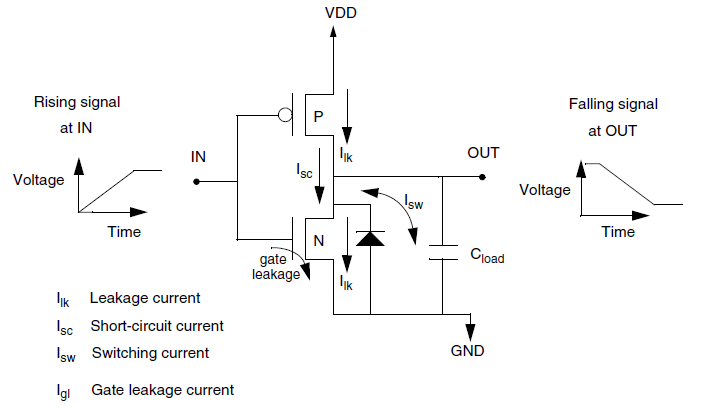
\includegraphics[width=\textwidth]{prime_time_power}
	\caption[Komponenten der Leistungsaufnahme]{Komponenten der Leistungsaufnahme \cite{primeTime2016}}
	\label{fig:prime_time_power}
\end{figure}
Mithilfe dieses Evalutionsablaufes sind die in diesem Kapitel evaluierten Ergebnisse entstanden.
\section{Testprogramme}
Um den Einfluss der Register-Adressen besser verstehen zu können wurden Assemblerprogramme entwickelt welche den Einfluss von Target-, Source1- und Source2-Register untersuchen.Hierbei sind diese in der Komplexität gestaffelt. In den folgenden Kapiteln wird nun auf die Ergebnisse der einzelnen Programme und deren Erkenntnisse eingegangen.
\subsection{Empirische Tests}
\label{cap:empirischeTests}
Um die aufgestellte Annahme, dass sich die Verlustleistung proportional zur Hamming-Distanz verhält, zu bestätigen, wurden zu Beginn Assemblerprogramme entworfen, die nur mit physikalischen bzw. festen Registern arbeiten.
Außerdem wurden vorerst der Best- und Worst-Case untersucht, um das maximale Optimierungspotenial zu ermitteln. Das Programm durchläuft dabei alle Möglichkeiten der Adress-Port-Zuweisung, dies testet zum einen die Register-Allokation und die damit verbundene Hamming-Distanz-Berechnung, zum andern werden alle Einflüsse der Register-Adressierung ermittelt. Da der Prozessor zwei Register-Files mit jeweils zwei Write- und vier Read-Ports aufweist, bestehen für die Target-Register vier und für die Source-Register 16 Möglichkeiten der Portzuweisung (siehe Tabelle \ref{lese-port} sowie \ref{fig::schreib-port}), dabei sind X2-Operationen ausgenommen. Im Worst-Case werden die Register so adressiert, dass die maximale Hamming-Distanz entsteht. Dabei wechseln die Adressen von 0 auf 31 welches der maximalen Hamming-Distanz von fünf entspricht. Damit keine Einflüsse durch Scheduling oder Daten entstehen, wurden Instruktionen manuell geschedult und den einzelnen Issue-Slots zugewiesen. Somit ist die Anordnung der Assemblerbefehlen für jeden Testfall identisch und der Einfluss ist somit entkoppelt. Im Falle der Datenabhängigkeiten wurden alle Register mit einer Null initialisiert und im Anschluss nicht verändert. Dadurch werden alle Instruktionen mit den selben Daten ausgeführt und somit besteht keine Abhängigkeit der Daten mehr.
Für den Fall des Best-Case wurde die Adresse nicht verändert und immer auf die Adresse 0 gelesen sowie geschrieben.
Das Power-Analyse-Tool zeigt nach dem ausführen des Workflows \ref{fig:flow_power_analyse} eine Übersicht über die Leistungsaufnahme des Prozessors an. Hierbei wird die Leistung in Internal-, Switching- und Leakage-Leistung aufgeteilt (siehe Abbildung \ref{best_power_hierarchy}). Die Leakage-Power ist hierbei so, dass alle Zeiten in der ein Transistor sperrt aufsummiert und mit den jeweiligen Transistor-Konfigurationen verrechnet werden. Bei der Leakage-Leistung handelt es sich somit um eine statische Verlustleistung. Hingegen sind Internal- und Switching-Leistung dynamische Verlustleistungen die von den Schaltvorgängen beeinflusst werden. Die Internal-Leistung inkludiert alle Leistungen die in einer Zelle durch das Laden von Kapazitäten verursachte werden. Dagegen werden in der Switching-Leistung die Verlustleistungen berücksichtigt die durch das Laden von externen Lastkapazitäten verursacht wurden.
Diese Leistungen werden über der Hierarchie der Module aufgeschlüsselt. Die letzte Spalte des Reports zeigt die Aufteilung der Leistungsaufnahme in Prozent. Dabei ist zu erkennen, dass das Register-File (vrf\_inst) mit 65,2\% die größte Leistungsaufnahme im Prozessor aufweist.

\begin{figure}[H] 
	\centering
	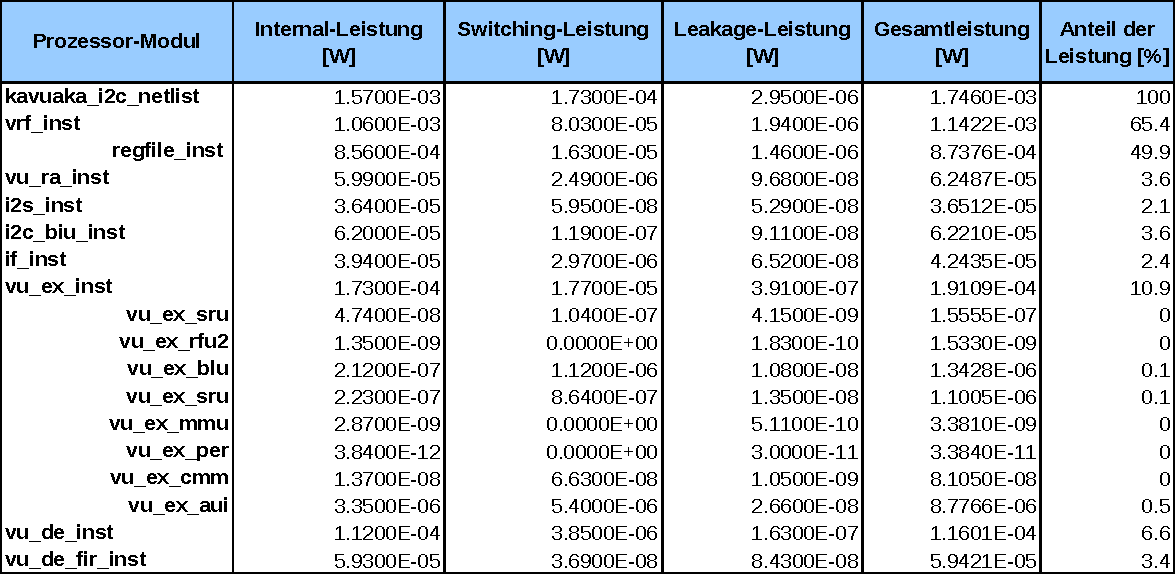
\includegraphics[width=\textwidth]{fig/best_hierarchy_report.pdf}
	\caption{Best-Case hierarchische Leistungsaufnahme}
	\label{fig:best_power_hierarchy}
\end{figure}

Aus beiden ermittelten Reports für den Worst- und Best-Case wurde die untenstehende Tabelle erzeugt (\ref{fig:best_powersave}). Dabei sind die Einträge in Prozent angegeben und zeigen eine deutliches Einsparungspotential. Außerdem sind alle Prozente auf die Gesamtleistung der entsprechenden Spalte bezogen. Das Augenmerk sollte hierbei auf die Switching-Leistung des Register-Files gelegt werden, denn hier wurden die Veränderungen in der Adressierung erzeugt. Dabei ist deutlich zu erkennen, dass eine maximal Einsparung von 38,65\% zu erreichen ist. Dies zeigt sehr deutlich, dass die Adressierung der Register eine Auswirkung auf die Verlustleistung hat. In den andern Modulen des Prozessors sind ebenfalls Verbesserungen zu erziehen, das liegt vor allem dran, dass die Register-Adressen ebenfalls in diesen angelegt sind. Bei Execution-Stage ist keine Verbesserung zu erzielen, da dort nur die Daten der jeweiligen Instruktion anliegen. Die Verbesserung der internen Leistungsaufnahme kann damit begründet werden, dass die Adressen ebenfalls Einfluss auf die interne dynamische Verlustleistung haben.
Durch das minimieren der Schaltaktivitäten hat zusätzlich den Vorteil, dass die Leakage-Leistung der Schaltung minimiert wird. Das Resultat der unterschiedlichen Adressierungen ist eine Gesamtverlustleistungseinsparung von 7,87\%.

\begin{figure}[H] 
	\centering
	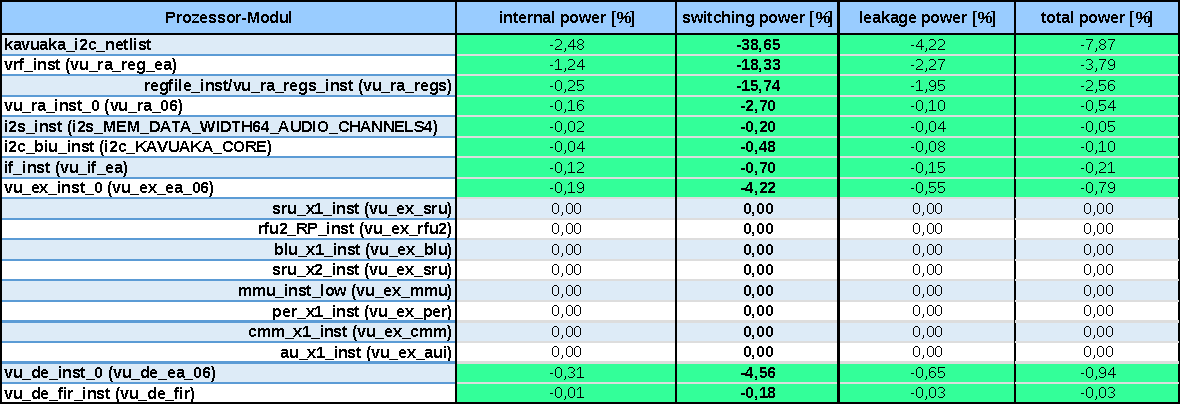
\includegraphics[width=\textwidth]{fig/best_worst_compare.pdf}
	\caption{Einsparungspotential Best-Worst-Case}
	\label{fig:best_powersave}
\end{figure}
\subsection{Synthetische Testprogramme}
Da nun bewiesen wurde, dass ein Zusammenhang zwischen Adressierung und Verlustleistung besteht, soll die Register-Allokation nun näher untersucht werden. Hierzu wurden synthetische Testfälle erstellt welche mit unterschiedlichen Adressierungen, aber selben Daten arbeiten. Dabei wurden vorerst die Register einzeln betrachtet. Um die einzelnen Ergebnisse vergleichen zu können wurden die Programme so entworfen, dass die Hamming-Distanzen für alle Testfälle identisch ausfallen. Das heißt die Schaltaktivitäten in den Lese- sowie Schreibports sind identisch und die Leistungen können somit verglichen werden. Ein Beispiel für ein solches Testprogramm, welches den Einfluss der Target-Register testet, finden sie im Codebeispiel \ref{code:target_switching_test}. Um die Source-Register vom Test zu entkoppeln, wurden die Adressen der Register, die nicht untersucht werden sollten nicht verändert. Dadurch entsteht keinerlei Schaltaktivität in den Adressleitungen. Gestartet wird die Berechnung der Hamming-Distanz immer mit der Adresse 0, da keine Aussage getroffen werden kann welche Adresse in der letzten SLM zugewiesen wurde.

\begin{algorithm}[H]
	\begin{algorithmic}[1]
		\STATE {:0 \textbf {ADD} V0R2 V0R0 V1R0 \hspace{50pt}:1 \textbf {OR} V0R2 V0R0 V1R0}
		\STATE {:0 \textbf {ADD} V0R0 V0R0 V1R0 \hspace{50pt}:1 \textbf {OR} V1R2 V0R0 V1R0}
		\STATE {:0 \textbf {ADD} V1R0 V0R0 V1R0 \hspace{50pt}:1 \textbf {OR} V0R2 V0R0 V1R0}
		\STATE {:0 \textbf {ADD} V1R2 V0R0 V1R0 \hspace{50pt}:1 \textbf {OR} V1R2 V0R0 V1R0}
		\STATE {:0 \textbf {ADD} V0R0 V0R0 V1R0 \hspace{50pt}:1 \textbf {OR} V0R0 V0R0 V1R0}
		\STATE {:0 \textbf {ADD} V0R2 V0R0 V1R0 \hspace{50pt}:1 \textbf {OR} V1R0 V0R0 V1R0}
		\STATE {:0 \textbf {ADD} V1R2 V0R0 V1R0 \hspace{50pt}:1 \textbf {OR} V0R0 V0R0 V1R0}
		\STATE {:0 \textbf {ADD} V1R0 V0R0 V1R0 \hspace{50pt}:1 \textbf {OR} V1R0 V0R0 V1R0}
		\caption{Codebeispiel Target-Register }
		\label{code:target_switching_test}
	\end{algorithmic}
\end{algorithm}

Dieser Test wurde für Adressen zwei, fünf, 24, 25 ,27 und 31 ausgeführt. Außerdem wurden Target, Source 1 und Source 2 getestet. Die untenstehenden Schaubilder(\ref{fig:source0_power}, \ref{fig:source1_power}, \ref{fig:target0_power} sowie \ref{fig:target1_power}) zeigen hierbei der Schaltleistung der verschiedenen Testfälle. Es ist schön zu erkennen, dass die Schaltleistungen der Lese- sowie Schreibports linear mit der Hamming-Distanz steigen. Außerdem sind die Graphen der Source-Register nahezu identisch, welches impliziert, dass die Adressen in den Lese-Ports eine identische Verlustleistung verursachen.\\

\begin{figure}[H]
	\centering
	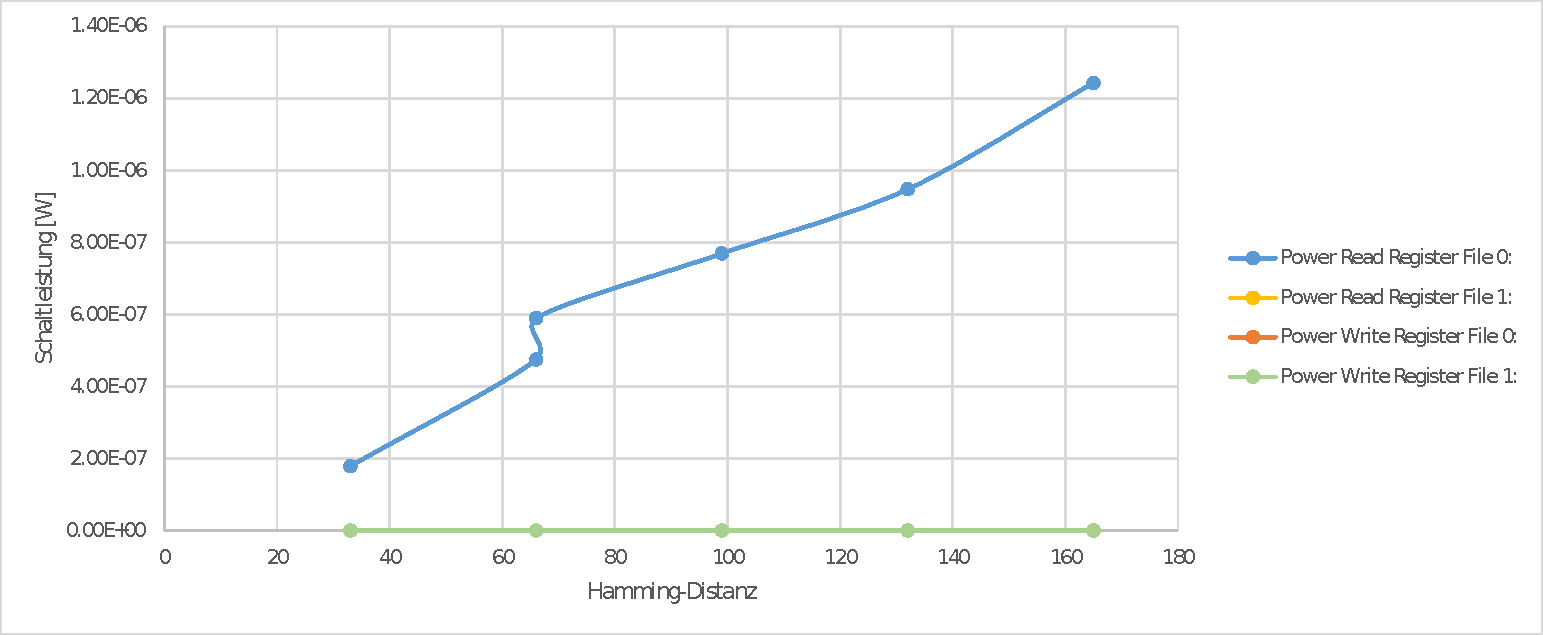
\includegraphics[width=\textwidth]{fig/source1_power.pdf}
	\caption{Schaltleistung Read Register File 0}
	\label{fig:source0_power}
\end{figure}
\begin{figure}[H]
	\centering
	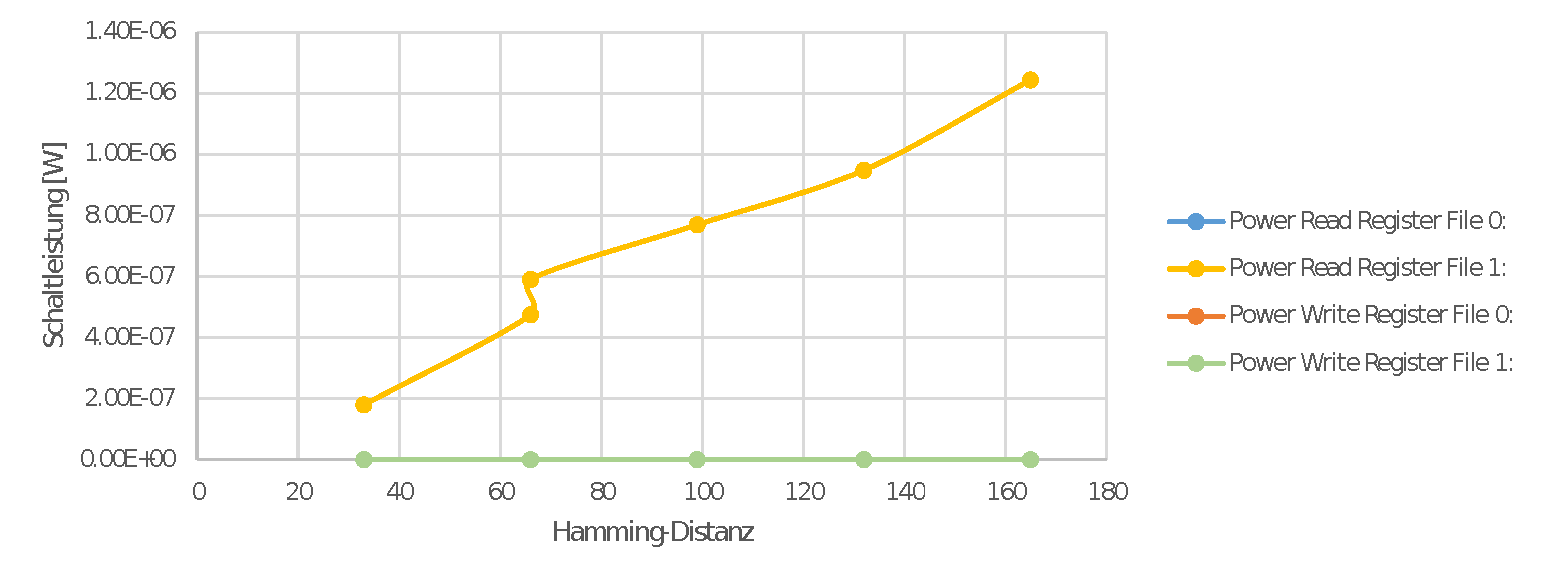
\includegraphics[width=\textwidth]{fig/source2_power.pdf}
	\caption{Schaltleistung Read Register File 1}
	\label{fig:source1_power}
\end{figure}
\begin{figure}[H]
	\centering
	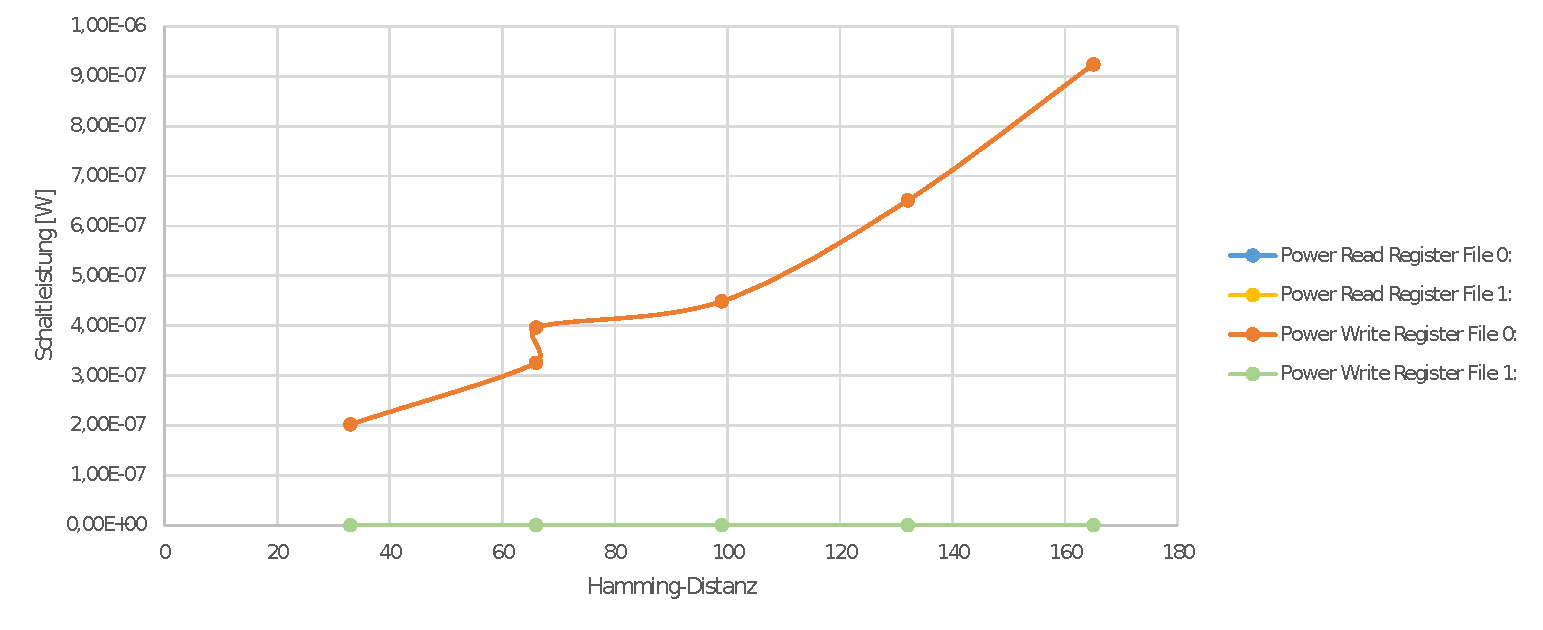
\includegraphics[width=\textwidth]{fig/register_eval_target_port0.pdf}
	\caption{Schaltleistung Write Register File 0}
	\label{fig:target0_power}
\end{figure}
\begin{figure}[H]
	\centering
	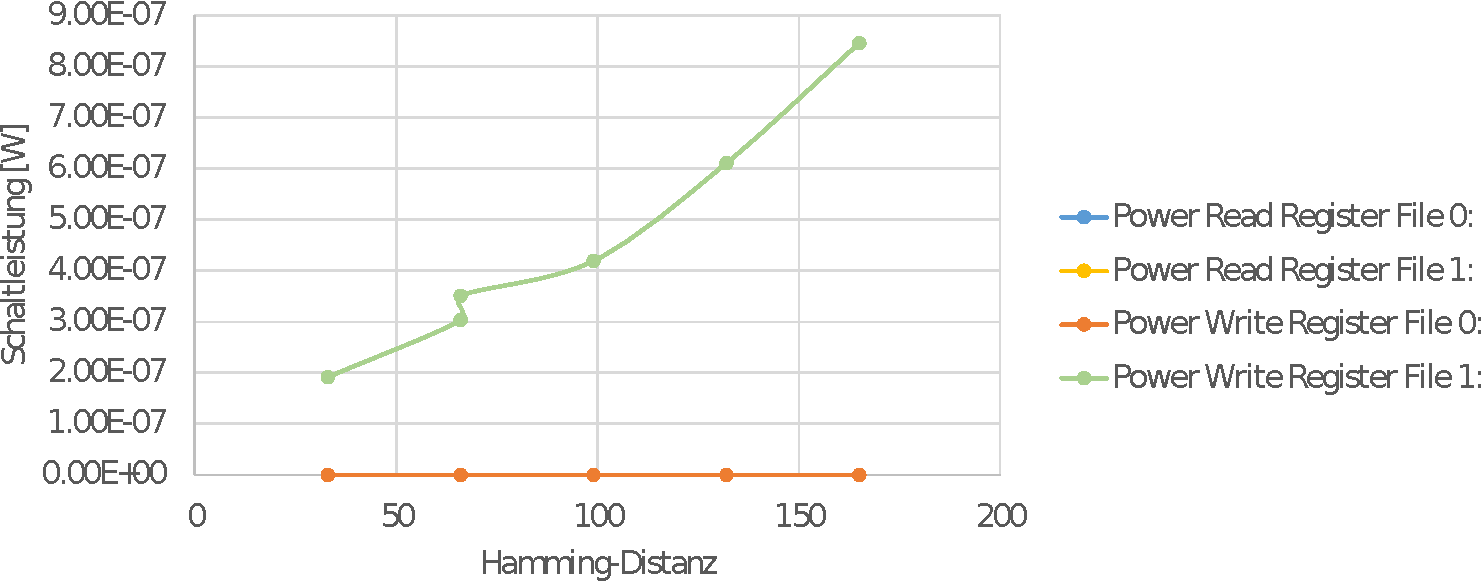
\includegraphics[width=\textwidth]{fig/register_eval_target_port1.pdf}
	\caption{Schaltleistung Write Register File 1}
	\label{fig:target1_power}
\end{figure}

Bei den Graphen ist ein Sprung der Leistung bei einer Hamming-Distanz von 64 auffällig. Dieser lässt sich dadurch erklären, dass zwar die Hamming-Distanzen der Testfälle mit den Register-Adressen fünf und 24 identisch sind, aber unterschiedliche Adressleitungen verwendet werden, welche eine größere Lastkapazität aufweisen. Durch die höhere Lastkapazität wird automatisch auch einer größere Leistung benötigt. Dieses Phänomen wird in Kapitel \ref{cap:lastkapa} näher untersucht und erläutert.\\

Nach dem die Register nun getrennt voneinander betrachtet und gezeigt wurde, dass die Adressen ca. die selbe Schaltleistungen in den Ports verursachen, soll nun das Verhalten beim gemeinsamen Schalten der Source- sowie Target-Register untersucht werden. Auch hierbei werden die Tests mit den selben Hamming-Distanzen für Lese- und Schreib-Ports ausgeführt. Das untenstehende Schaubild \ref{fig:source_target_power} zeigt auch hier, dass ein linearer Verlauf erkennbar ist.

\begin{figure}[H]
	\centering
	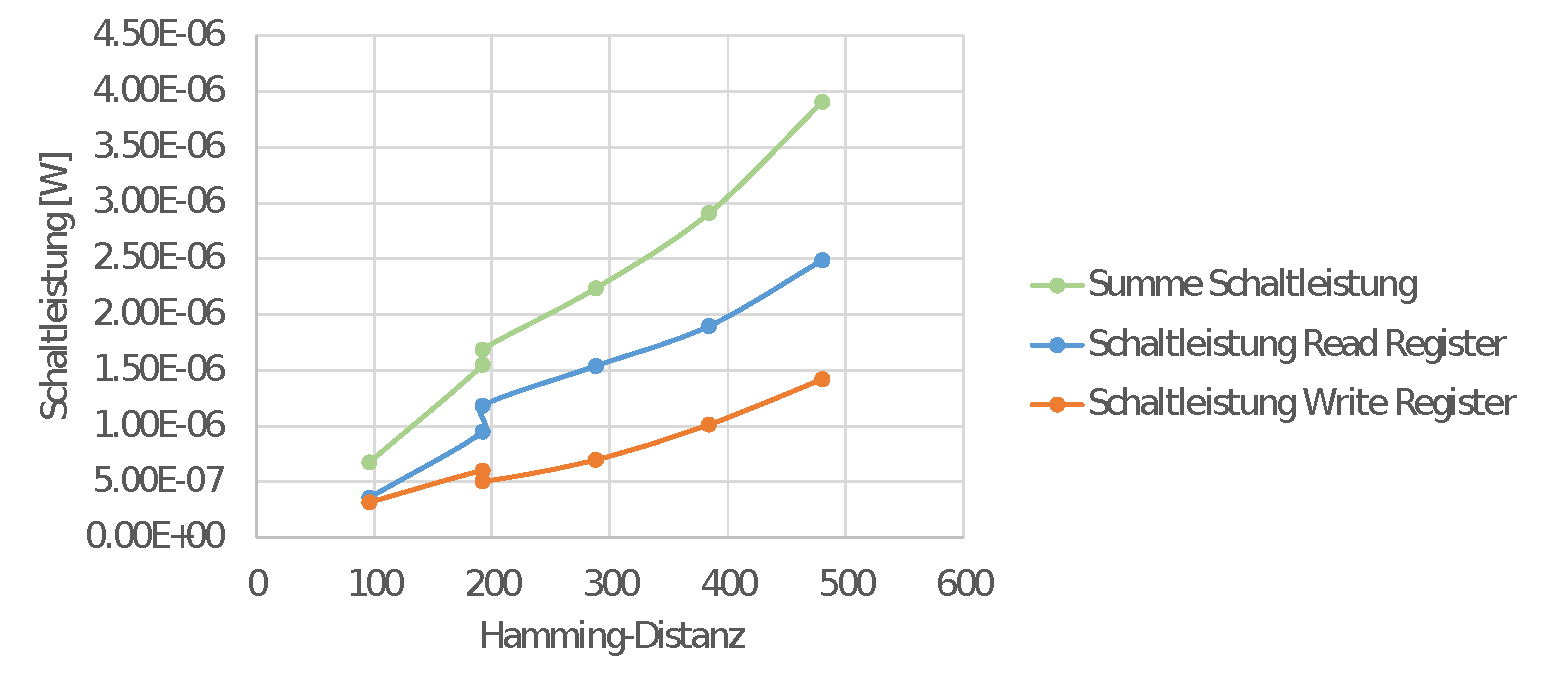
\includegraphics[width=\textwidth]{fig/source_target_power.pdf}
	\caption{Schaltleistung Read+Write Register}
	\label{fig:source_target_power}
\end{figure}

Außerdem zeigt Abbildung \ref{fig:total_power_source_target} die Gesamtleistung des Prozessors über der Hamming-Distanz. Auch hier ist eine deutliche Verbesserung erkennbar welche sich ebenfalls linear zur Hamming-Distanz verhält.

\begin{figure}[H]
	\centering
	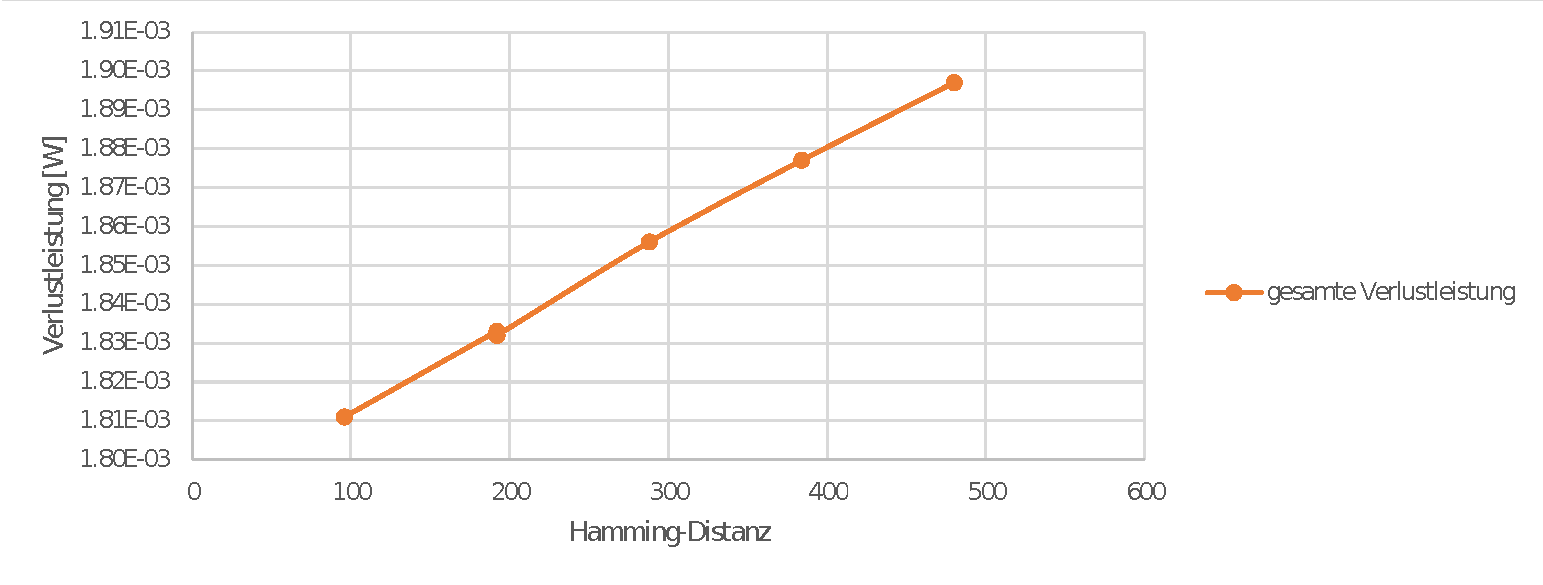
\includegraphics[width=\textwidth]{fig/total_power_source_target.pdf}
	\caption{gesamte Verlustleistung des Prozessors}
	\label{fig:total_power_source_target}
\end{figure}

Um nun ebenfalls den Einfluss der Daten auf die Verlustleistung zu ermitteln wurden die oben genannten Programme mit Zufallszahlen ausgeführt. Hierzu wurden vorerst alle Register mit zufälligen Zahlen initialisiert und im Anschluss die oben beschriebenen Funktionen abgearbeitet. Diese Änderung verursacht einen Anstieg der Verlustleistung, jedoch ist zu untersuchen, ob die Einsparung durch die Adressierung dominiert. Hierzu wurden die Testfälle mehrere Male durchlaufen, so dass die Werte aussagekräftig sind. Das untenstehende Schaubild \ref{fig:random_data_total_power} zeigt hierbei die Verläufe des Testfalls mit null initialisierten Daten in rot und mit Zufallszahlen befüllten Registern in blau. Es ist deutlich zu erkennen, dass trotz einer Abhängigkeit der Daten die Optimierung der Adressen dominiert und die Verlaufe sich ähneln.

\begin{figure}[H]
	\centering
	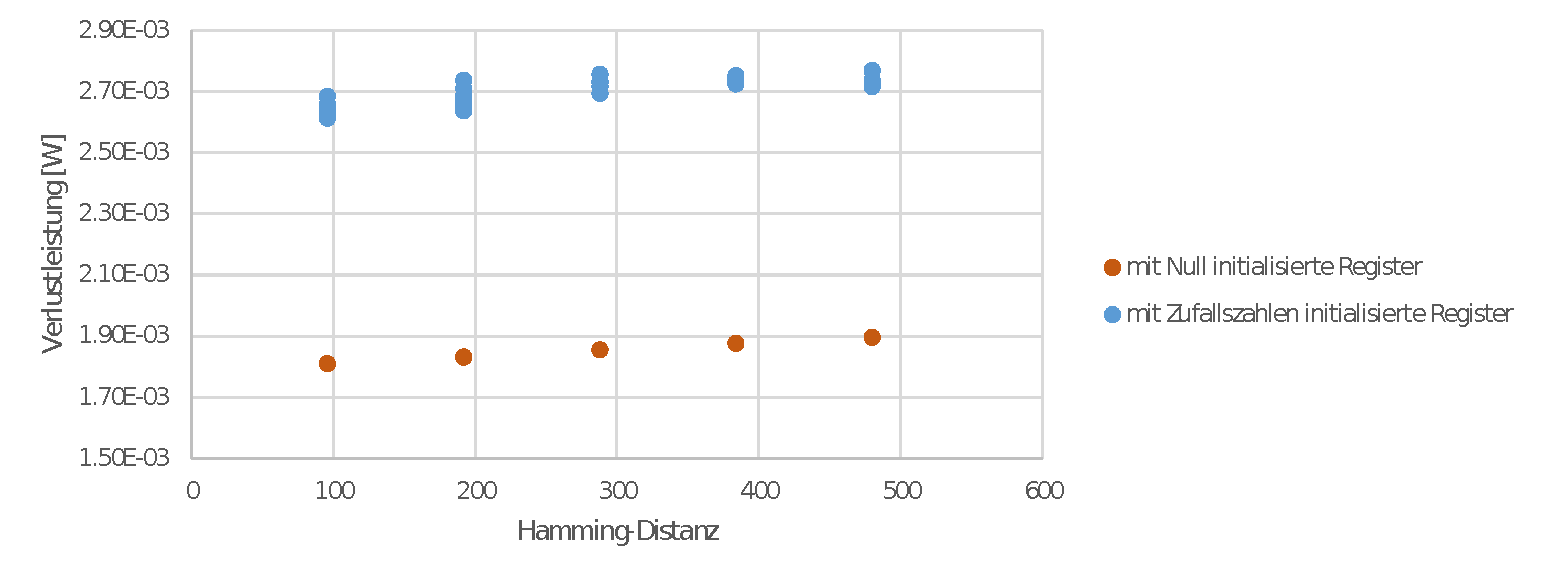
\includegraphics[width=\textwidth]{fig/random_data_total_power.pdf}
	\caption{Einfluss der Daten auf die gesamte Verlustleistung}
	\label{fig:random_data_total_power}
\end{figure}


\subsection{Heuristik}
\label{chap:eval_heuristik}
Da nun die Abhängigkeiten der Register-Adressierung zu der Verlustleistung bewiesen wurde, wie diese durch den Einsatz von virtuellen Registern und der neu implementierten Heuristik verbessert werden kann. Hierzu werden wie in Kapitel \ref{cap:empirischeTests} Assemblerprogramme entworfen welche manuell geschedult sind und die Register mit Null initialisiert werden. Der unterschied zu den empirischen Testprogrammen liegt darin, dass nun ebenfalls virtuelle Register verwendet werden.
Dies hat zur folge, dass die Register-Allokation ein geeignete Zuweisung finden muss und somit die Schaltaktivität der Adresse minimieren kann. Das Testprogramm belegt vorerst durch physikalische Adressierung eine gewisse Anzahl an Registern vor und blockiert diese somit für die Verwendung von virtuellen Register.(Siehe Abbildung \ref{fig:heuristik_eval}, blau hinterlegte Felder)
Nach dem die Register-Files vorbelegt wurden, wird mit der Zuweisung von virtuellen Registern begonnen. Ab diesem Punkt ergeben sich Veränderungen in der Register-Allokation. Je nach gewähltem Verfahren, wird nach den optimalen physikalischen Registern mit unterschiedlichen Algorithmen gesucht. 

\begin{figure}[H] 
	\centering
	\includesvg[width=\textwidth]{heuristik_eval}
	\caption{Heuristik Evaluation}
	\label{fig:heuristik_eval}
\end{figure}
Das Schaubild zeigt hierbei den Vergleich der alten zur neuen Heuristik. Die blockierten Register-Adressen sind blau hinterlegt, die von den Algorithmen ausgewählten Register-Adressen sind rot gekennzeichnet. Durch die beiden unterschiedlichen Verfahren ergibt sich ein Unterschied von 11 Schaltvorgängen in den Adress-Leitungen. Damit dieser in der Verlustleistung deutlicher zu erkennen ist, wird die Zuweisung der virtuelle Register zehn mal wiederholt. Dadurch ergibt sich ein Differenz der Hamming-Distanzen von 101, da durch das wiederholte Ausführen der Allokation die Zuweisung mit unterschiedlichen Adressen gestartet wird.
Damit der Zusammenhang von Verlustleistung zu Schaltaktivität zu erkennen ist, wurden fünf Testfälle mit unterschiedlichen Hamming-Distanzen erzeugt. Hierbei variieren die Hamming-Distanzen im Bereich zwischen 101 und 500 Das Schaubild XXX zeigt den Verlauf der Verlustleistung der Adress-Ports über der Hamming-Distanz. 

SChaubild SChaltleistung heuristik neu 

Die Evaluation der Heuristik zeigt, dass für die entwickelten synthetischen Testfälle die neue Heuristik eine durchschnittliche Verbesserung der Hamming-Distanz von XXX\% erzielt werden kann. Diese Optimierung spiegelt sich ebenfalls in der Schaltleistung des Prozessor wieder.(siehe Abbildung XXX).

 Schaubild Gesamtleistung Heuristik neu

Die Tabelle XXX zeigt die Optimierung der Verlustleistung in den einzelnen Modulen des Prozessors gegenüber der alten Implementierung. Hierbei sind alle Werte in Prozent angegeben und beziehen sich auf die Gesamtleistungen der Spalten. Auch hier ist zu erkennen das deutliche Einsparungen in den Register-Files generiert werden konnten. Dabei wurde die Schaltleistung im Register-File gegenüber der alten Heuristik um XXX\% verbessert. Die gesamte Verlustleistung wurde um XXX\% optimiert. 

Tabelle Prozent alt neu

\subsection{Genetischer Algorithmus}
Da die Heuristik wie bereits in Kapitel \ref{sec:genetischerAlgorithmus} erwähnt, nur die Target-Register auf Schaltaktivität minimiert werden, wird nun die Verbesserung der Verlustleistung durch zusätzliches optimieren der Source-Register untersucht.
Bei der Evaluation wurde ein genetischer Algorithmus verwendet, der mit einer Heuristik eine Startpopulation berechnet um eine schnelle Konvergenz gegen ein Minimum zu garantieren. Außerdem wird die Mutationswahrscheinlichkeit dynamisch angepasst. Als Fitness-Funktion wird die Multiplikation aus Hamming-Distanz und Lastkapazität gewählt. 
Um den Optimierungsgrad gegenüber der alten und neuen Heuristik vergleichen zu können, wurde der genetische Algorithmus mit den selben synthetischen Testprogrammen wie in Kapitel \ref{chap:eval_heuristik} getestet.
Da der genetische Algorithmus zufallsgesteuert ist, variieren die Ergebnisse stark. Um dennoch eine Aussage über die Verbesserung gegenüber der Heuristik treffen zu können, wurden die Testfälle fünf mal ausgeführt. Das Schaubild  \ref{fig:eval_genetic_total_power} zeigt, wie stark die Ergebnisse der gesamten Verlustleistung untereinander variieren. Es ist jedoch deutlich zu erkennen, dass in jedem Fall eine Verbesserung der Verlustleistung erzielt werden konnte.

\begin{figure}[H]
	\centering
	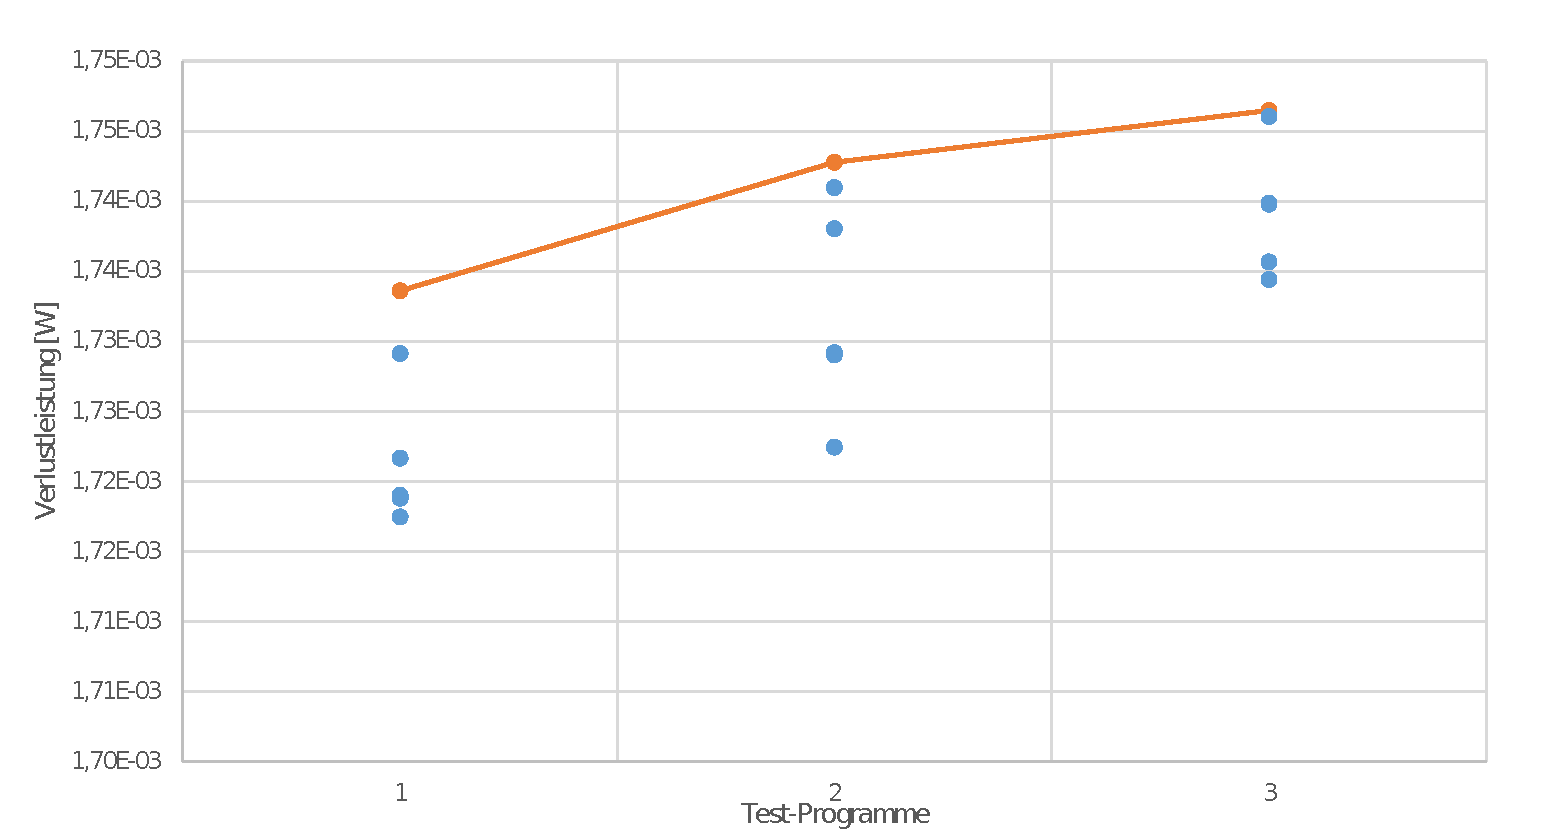
\includegraphics[width=\textwidth]{fig/eval_genetic_total_power.pdf}
	\caption{Gesamtverlustleistung genetischer Algorithmus vs. Heuristik}
	\label{fig:eval_genetic_total_power}
\end{figure}

In der besten Variante des genetischen Algorithmus, ist eine Verbesserung der Hamming-Distanz von 48,64\% zu erreichen. Diese verursacht eine Optimierung der Schaltleistung der Adressleitungen um 50,38\% und der Gesamtleistung um 0,62\%. Die komplette Einsparung fällt relativ gering aus, jedoch ist hervorzuheben, dass diese Optimierung komplett \glqq kostenfrei \grqq und ohne Veränderung der Hardware erzielt werden kann.

%Im unten stehenden Schaubild XXX wird der Mittelwert der Testfälle gegenüber der alten Heuristik veranschaulicht. 
%
%Mittelwert genetischer Algo gegenüber alter heuristik

Auch hier zeigt ein prozentualer Vergleich der Verlustleistungen des kompletten Prozessors eine deutliche Verbesserung der Schaltleistung in den Register-Files. In diesem Fall wird die beste Variante des genetischen Algorithmus mit der Heuristik verglichen. Die Tabelle zeigt eine Verbesserung der Schaltleistung um 7,78\%. Die Verlustleistung die durch die Leakage-Ströme verursacht wurden sind um zwei bzw. drei Zehnerpotenzen kleiner als die Verlustleistungen die durch die Schaltvorgänge hervorgerufen werden. Aus diesem Grund werden dies Vernachlässigt. Eine Verschlechterung der Leakage-Leistung ist damit zu erklären, dass die Signale des Prozessors für längere Zeit ihre Pegel halten. Da die Leakage-Leistung nur dann auftritt, wenn kein Wechsel der Pegel stattfindet, wird im Fall einer optimierten Schaltleistung die Leakage-Leistung ungewollt erhöht.
Die prozentuale Veränderung der Internal-Leistung liegt im sehr niedrigen Prozentbereich. 

\begin{figure}[H]
	\centering
	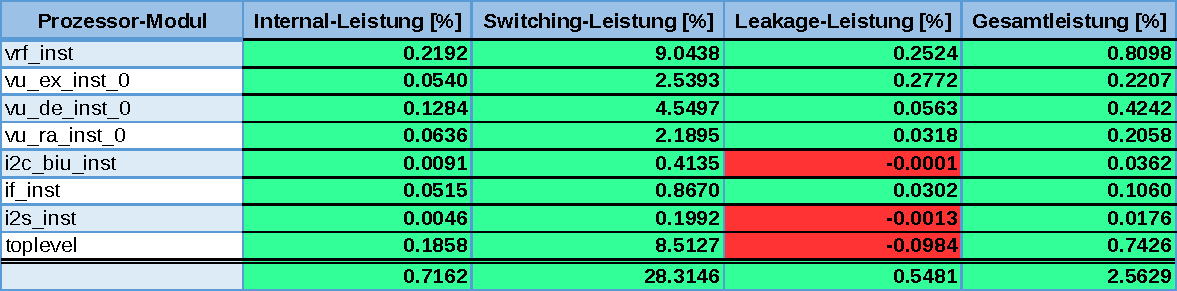
\includegraphics[width=\textwidth]{fig/power_percent_genetic.pdf}
	\caption{Prozentuale Verbesserung der Verlustleistung}
	\label{fig:power_percent_genetic}
\end{figure}



\section{Hörgerätalgorithmen}
\label{sec:testprogamme}
Um den implementierten Code zu testen und eine reelle Einsparung der Verlustleistungsreduktion zu ermitteln wurden die folgenden Assembler-Programme verwendet. Dabei handelt es sich um Programme die eine häufig Anwendung in Hörgerät-Prozessoren finden. Ausschlaggebend für die Wahl war die Anzahl der verwendeten virtuellen Registern da mit einer hohen Zahl das Verbesserungspotential der Register-Allokation steigt.
\subsection{fft floating Point}

\subsection{Beamforming}
Der Beamforming-Algorithmus wird eingesetzt um eine Positionsbestimmung von Schallwellen im Raum durchzuführen und somit eine Ein- bzw Ausblendung von verschiedenen Geräuschen zu gewährleisten und so das Hörerlebnis zu steigern. 

\subsection{emulated floating Point}
Da der verwendete Prozessor keine floating Point Variablen unterstützt, besteht ein Algorithmus der diese emuliert. 


\subsection{Einfluss des Register-Daten auf die Verlustleistung}
In Kapitel \ref{cap:empirischeTests} wurde bereits der Einfluss der Daten auf die Verlustleistung ermittelt. Da sich nun jedoch eine Verschlechterung der Register-File-Leistung bei besserer Adressierung in den realen Testfällen ergibt wurden die Datenabhängigkeit nochmals überprüft. Dabei ergab sich, dass auf Grund des Verhalten des Adress-Decoders eine Veränderung der Daten verursacht wird. Da die Adressen über einen Adress-Decoder decodiert werden müssen und dieser nicht direkt alle Bits auf einmal umschalten kann, liegen kurze Zeit, Daten aus anderen Adressen an den Daten-Leitungen an. Dies Verursacht dort eine Schaltleistung welches die Verbesserung durch die Adressierung aufhebt.
Um dieses Verhalten und die Funktion des Decoders besser nachzuvollziehen wurden nun weitere Testfälle generiert. Diese befüllen wie in Kapitel \ref{cap:empirischeTests} alle Register mit zufälligen Daten. Der unterschied liegt jedoch darin, dass die Instruktionen in allen Testfällen mit den selben Zufallsdaten arbeiten, so dass immer die selben Daten in die entsprechenden Register geschrieben werden.

Hierbei war zu erkennen, 

\section{Einfluss der Lastkapazität}
 \label{cap:lastkapa}
Wie bereits in Kapitel \ref{cap:empirischeTests} erwähnt besteht eine Abhängigkeit zwischen Lastkapazität und Verlustleistung. Dies lässt sich auf die Formel der dynamischen Verlustleistung zurückführen \ref{eq:dynVerlustleistung}, laut dieser steigt die Verlustleistung linear mit der Lastkapazität.
Das untenstehende Schaubild \ref{fig:read_port_mux} zeigt wie die Daten aus den Registern an die Read-Ports angelegt werden. Hierbei ist jedes Bit der Register-Adresse für das Schalten eines Multiplexers zuständig. Besteht nun der Fall, dass ein Register mit einer Adresse von 31 ausgelesen werden soll, so müssen alle Multiplexer durchschalten. Dadurch werden die Daten des Registers an den Verwendeten Register-Port weitergeleitet. Wird im Gegensatz hierzu eine niedrige Adresse beispielsweise 0 angefragt, so muss keiner der Multiplexer schalten. Das Signal liegt direkt an dem Read-Port an. Aus diesem Grund benötigen die oberen Adressleitungen mehr Verlustleistung da das Signal eine höhere Lastkapazität aufweist. Dies lässt sich ebenfalls in den Power-Reports nachvollziehen. Dort ist deutlich zu erkennen, dass die oberen Register-Adressen eine höhere Lastkapazität aufweisen. 
\begin{scriptsize}
	\begin{figure}[htbp] 
		\centering
		\includesvg[width=\textwidth]{Read-Port-Mux}
		\caption{Read-Port Multiplexer}
		\label{fig:read_port_mux}
	\end{figure}
\end{scriptsize}

Aus diesem Grund wurde die Fitness Funktion des Genetischen Algorithmus so angepasst, dass die Lastkapazität zusätzlich berücksichtigt wird.
